\section{Numerical Experiment}
\label{sec:4}
In this section, we apply various methods to solve the LP form of optimal transport \ref{lp} and the entropic regularization of optimal transport \ref{equ:kl}. All of the numerical experiments are conducted on an Intel Core i7-6500U Processor with 2 cores and 4 threads.

\subsection{Datasets of Optimal Transport}
We perform the numerical experiments on various datasets, including randomly generated data, DOTmark\cite{DOTmark}, ellipse example \cite{multiscale}, Caffarelli's example \cite{multiscale} and Gaussian mixture model. 

\subsubsection{Randomly generated data}
In order to make the feasible set not empty, we first generate a random matrix $R\in \mbR^{m\times n}$, where $R_{i,j}\sim \mcN(0,1)\, i.i.d.$. and then generate $\mu_i, \nu_j$ by
$$
\mu_i=\frac{\sum_{j=1}^n|R_{i,j}|}{\sum_{i=1}^m\sum_{j=1}^n|R_{i,j}|}, \, \forall i=1, 2, \dots m\\
$$
$$
\nu_j=\frac{\sum_{i=1}^m|R_{i,j}|}{\sum_{i=1}^m\sum_{j=1}^n|R_{i,j}|}, \, \forall j=1, 2, \dots n\\
$$
It is easy to verify that $\sum_{i=1}^m\mu_i=\sum_{j=1}^n\nu_j=1$. We then generate $C_{i,j} \sim \mcN(0,1)\, i.i.d.$. We denote $C_{\mathrm{min}}=\min_{i,j}C_{i,j}$ and let $C_{i,j}=C_{i,j}-C_{\mathrm{min}}$ to ensure $C_{i,j}\geq 0$. 

\subsubsection{DOTmark}
DOTmark \cite{DOTmark} provides $10$ classes of $10$ different images, each of which is available at the different resolutions from $32\times32$ to $512\times512$. Suppose we select two images $x$ and $y$ with same resolution $l\times l$ from one class. The corresponding parameter for the standard form of LP is given in the following way: $m=n=l^2$, $\mu_i=x_i$, $\nu_j=y_j$ and $C_{i,j}=\|x_i-y_j\|_p$, where $(x_i)_{1\leq i\leq m}$ and $(y_j)_{1\leq j\leq n}$ form a regular square grid in $\mbR^2$. In practice, we take $p=2$. In solving this LP, we actually calculate the Wasserstein distance between $x$ and $y$.

\subsubsection{Ellipse Example}
The ellipse example consists of two uniform samples, source and target data set, of size $n$ from the unit circle with normal distributed noise added with zero mean and deviation 0.1. Slightly different from that in the paper \cite{multiscale}, we construct the source data example by scaling in the x-Axis by 2.0 and in the y-Axis by 0.5. The target data sample is then scaled in the x-Axis by 0.5 and y-Axis by 2.0. The corresponding parameter for the standard form of LP is as follows. $m = n$, $\mu_i=1, \nu_i=1(i=1, ..., n)$ and $C_{i, j}=\|x_i-y_j\|_2$, which is the Euclidean distance between two points $x_i$ and $y_j$. Figure \ref{ellipse} gives an example. 
\begin{figure}[h]
\centering
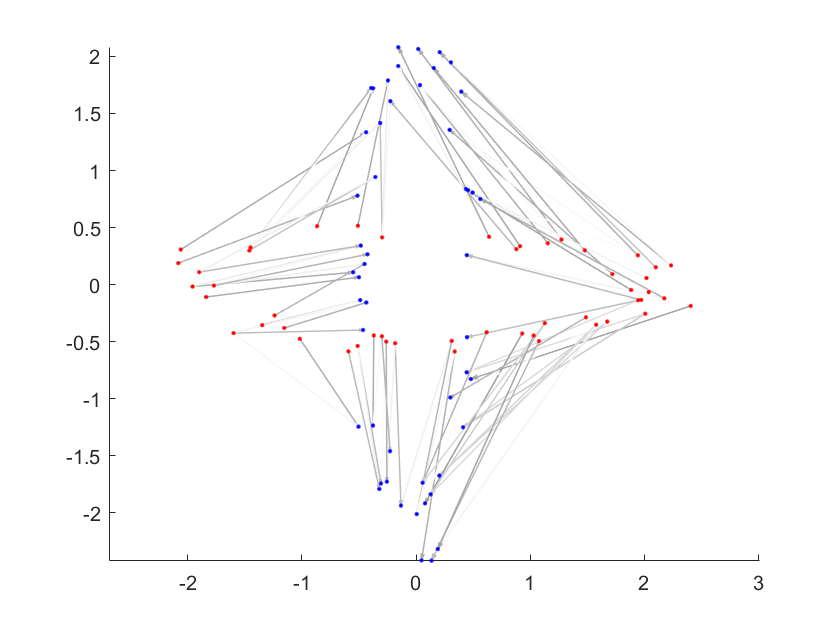
\includegraphics[width=12cm]{final/ellipse1.png}
\caption{An Ellipse Example with sample size $n=50$. The darker the line, the greater the $\pi_{i, j}$.}
\label{ellipse}
\end{figure}

\subsubsection{Caffarelli's Example}
This example, mentioned in \cite{multiscale}, consists of two uniform samples on $[-1, 1]^2$ of size $n$. Then any point outside the unit circle are then discarded. The source and target data sample is split along the x-Axis at 0 and shifted by -2 and +2, respectively. Note that the true number of points may be less than $n$. When $n$ is large, about $\frac{\pi}{4}n$ points are preserved. For ease of notation, we still assume there are $n$ points. The corresponding parameter for the standard form of LP is as follows. $m = n$, $\mu_i=1, \nu_i=1(i=1, ..., n)$ and $C_{i, j}=\|x_i-y_j\|_2$, which is the Euclidean distance between two points $x_i$ and $y_j$. Figure \ref{caff} gives an example.
\begin{figure}[h]
\centering
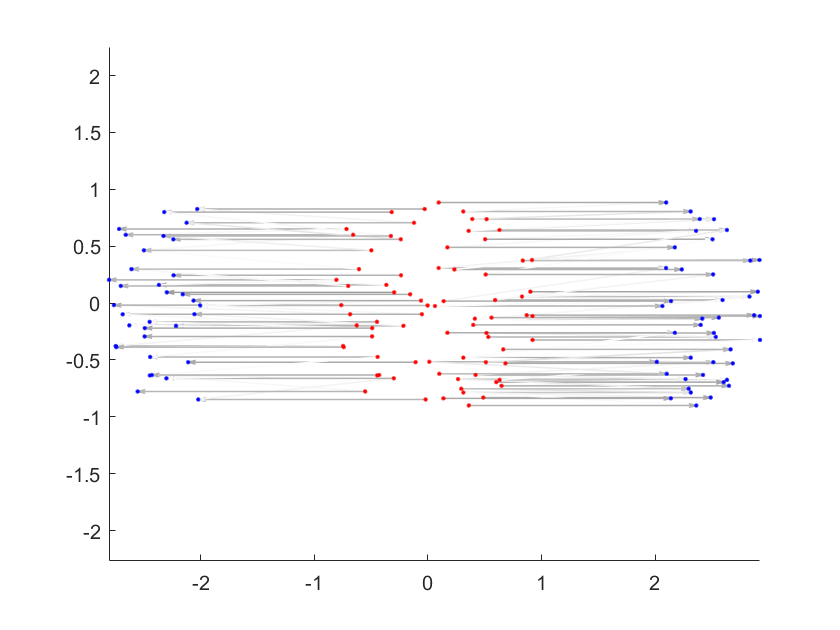
\includegraphics[width=12cm]{final/caff1.png}
\caption{An Caffarelli's Example with sample size $n=50$. The darker the line, the greater the $\pi_{i, j}$.}
\label{caff}
\end{figure}

\subsubsection{Gaussian Mixture Model}
Suppose $p_\mu$ and $p_\nu$ are the probability density function of two different Gaussian mixture models and $N$ is the number of discrete points. In this example, $\mu$ and $\nu$ are the normalized discrete distribution of Gaussian mixture models, which satisfy
$$
\mu_i=\frac{p_\mu(\frac{i-1}{N-1})}{\sum_{i=1}^Np_\mu(\frac{i-1}{N-1})}, \quad \nu_j=\frac{p_\nu(\frac{j-1}{N-1})}{\sum_{j=1}^Np_\nu(\frac{j-1}{N-1})}
$$
And $C_{i,j}=|i-j|$. 

\subsection{Different methods on Mosek and Gurobi}
`prim', `dual', `int' represent primal simplex, dual simplex and interior point method respectively. `(M)' means Mosek, `(G)' means Gurobi. For each method, we record the time and the number of iteration it takes and evaluate their performance. We examine the accuracy of the solution $\pi$ by the value of the objective function ('objval') 
$$
\sum_{i=1}^m\sum_{j=1}^nC_{i,j}\pi_{i,j}
$$
and the violation of the constraints ('vltcst') 
$$
\sum_{i=1}^m|\mu_i - \sum_{j=1}^{n}\pi_{i, j}| + \sum_{j=1}^n|\nu_j-\sum_{i=1}^m\pi_{i, j}|$$
In the table, we only give the exact value of `objval' for prim(M). In `objval' of other methods, we give its relative difference to prim(M). Namely, if `objval' for prim(M) is $f_1$ and `objval' for prim(G) is $f_2$, in `objval' of prim(G), we give $\frac{f_1-f_2}{f_1}$. 

\subsubsection{Randomly generated data}
For simplicity, we only consider the case when $m=n$. We take $m=128,256,512,1024$.  

\begin{table}[h]
\caption{Perfomance of mosek and gurobi on randomly generated data}
\label{RGD_mg}
\centering
\begin{tabular} {|c|c|c|c|c|c|c|c|} 
\hline
\multicolumn{2}{|c|}{method}&prim(M)&dual(M)&int(M)&prim(G)&dual(G)&int(G)\\\hline
\multirow{4}*{\makecell{$m=128$\\$n=128$}} 
&time(s)& 0.05 & 0.04 & 0.08 & 0.07 & 0.03 & 0.08 \\\cline{2-8}
&iter& 1488 & 220 & 13 & 3101 & 204 & 13 \\\cline{2-8}
&objval& 1.36e+00 & -6.08e-06 & -6.08e-06 & -6.08e-06 & -6.08e-06 & -6.08e-06 \\\cline{2-8}
&vltcst& 1.11e-05 & 5.55e-17 & 1.14e-10 & 4.94e-17 & 4.94e-17 & 4.94e-17 \\\hline
\multirow{4}*{\makecell{$m=256$\\$n=256$}} 
&time(s)& 0.21 & 0.18 & 0.33 & 0.20 & 0.14 & 0.30 \\\cline{2-8}
&iter& 4708 & 480 & 13 & 9252 & 437 & 15 \\\cline{2-8}
&objval& 1.63e+00 & -1.90e-05 & -1.90e-05 & -1.90e-05 & -1.90e-05 & -1.90e-05 \\\cline{2-8}
&vltcst& 3.62e-05 & 4.99e-17 & 1.05e-10 & 7.81e-18 & 6.51e-18 & 7.81e-18 \\\hline
\multirow{4}*{\makecell{$m=512$\\$n=512$}} 
&time(s)& 0.95 & 1.38 & 1.99 & 1.17 & 0.63 & 2.06 \\\cline{2-8}
&iter& 11742 & 472 & 15 & 32211 & 2266 & 19 \\\cline{2-8}
&objval& 1.57e+00 & -4.76e-05 & -4.76e-05 & -4.76e-05 & -4.76e-05 & -4.76e-05 \\\cline{2-8}
&vltcst& 9.14e-05 & 1.73e-16 & 1.44e-12 & 7.42e-17 & 7.42e-17 & 7.42e-17 \\\hline

\multirow{4}*{\makecell{$m=1024$\\$n=1024$}} 
&time(s)& 5.39 & 11.95 & 11.37 & 6.28 & 3.13 & 12.32 \\\cline{2-8}
&iter& 28914 & 2299 & 18 & 108153 & 6020 & 23 \\\cline{2-8}
&objval& 1.94e+00 & -1.21e-04 & -1.21e-04 & -1.21e-04 & -1.21e-04 & -1.21e-04 \\\cline{2-8}
&vltcst& 2.31e-04 & 3.51e-16 & 2.85e-11 & 4.68e-17 & 4.66e-17 & 4.68e-17 \\\hline

\end{tabular}
\end{table}

From Table \ref{RGD_mg}, we can see on Mosek, dual simplex method and interior point method take much more time than primal simplex does, especially when $m, n$ are large. But on Gurobi, dual simplex method is the fastest method and the time primal simplex method takes is close to the time interior point takes. Interior point method takes much smaller number of iterations than  We can observe that compared to other methods, primal simplex method on Mosek gets the largest value of objective function and the largest value of the violation of constraints. On Mosek, dual simplex methods achieves the lowest value of `vltcst', which partly explains why it takes the longest time. On Gurobi, the solution from all methods satisfies constraints perfectly.

\subsubsection{DOTmark}
We then test the performance of Mosek and Gurobi on DOTmark \cite{DOTmark}. We number the classes of DOTmark with the order of alphabet in the following way.
\begin{table}[!htp]
\centering
\begin{tabular}{|c|c|c|c|c|}
\hline
CauchyDensity&ClassicImages&GRFmoderate&GRFrough&GRFsmooth\\\hline
1&2&3&4&5\\\hline
LogGRF&LogitGRF&MicroscopyImages&Shapes&WhiteNoise\\\hline
6&7&8&9&10\\\hline
\end{tabular}
\end{table}

We test on pictures with resolution $32\times32$. 
\begin{table}[htbp]
\caption{Perfomance of mosek and gurobi on DOTmark}
\label{DOTmark_mg}
\centering
\begin{tabular} {|c|c|c|c|c|c|c|c|} 
\hline
Class No.&method&prim(M)&dual(M)&int(M)&prim(G)&dual(G)&int(G)\\\hline
\multirow{4}*{1} 
&time(s)& 5.53 & 52.84 & 11.34 & 5.17 & 6.49 & 10.51 \\\cline{2-8}
&iter& 23489 & 13515 & 16 & 74691 & 58692 & 17 \\\cline{2-8}
&objval& 1.75e+01 & -1.54e-05 & -1.53e-05 & -1.53e-05 & -1.54e-05 & -1.53e-05 \\\cline{2-8}
&vltcst& 2.34e-05 & 3.28e-16 & 5.53e-12 & 1.48e-17 & 2.11e-17 & 2.53e-17 \\\hline
\multirow{4}*{2} 
&time(s)& 5.76 & 26.44 & 11.39 & 4.95 & 4.57 & 11.12 \\\cline{2-8}
&iter& 22163 & 7634 & 16 & 85161 & 24036 & 17 \\\cline{2-8}
&objval& 6.27e+00 & 6.43e-07 & 6.43e-07 & 6.43e-07 & 6.43e-07 & 6.43e-07 \\\cline{2-8}
&vltcst& 2.67e-05 & 2.37e-16 & 1.92e-11 & 8.57e-18 & 1.01e-17 & 8.81e-18 \\\hline
\multirow{4}*{3} 
&time(s)& 5.12 & 26.71 & 11.12 & 4.76 & 3.79 & 10.43 \\\cline{2-8}
&iter& 21240 & 7395 & 16 & 81109 & 16455 & 15 \\\cline{2-8}
&objval& 4.07e+00 & 2.50e-05 & 2.50e-05 & 2.50e-05 & 2.50e-05 & 2.50e-05 \\\cline{2-8}
&vltcst& 2.89e-05 & 3.56e-17 & 6.41e-14 & 1.11e-17 & 8.73e-18 & 1.12e-17 \\\hline
\multirow{4}*{4} 
&time(s)& 5.09 & 19.64 & 11.11 & 5.10 & 3.01 & 10.73 \\\cline{2-8}
&iter& 22063 & 4493 & 17 & 88412 & 7513 & 16 \\\cline{2-8}
&objval& 1.48e+00 & 1.69e-05 & 1.69e-05 & 1.69e-05 & 1.69e-05 & 1.69e-05 \\\cline{2-8}
&vltcst& 2.77e-05 & 9.29e-17 & 9.24e-11 & 1.56e-17 & 1.38e-17 & 1.59e-17 \\\hline
\multirow{4}*{5} 
&time(s)& 5.17 & 37.87 & 10.59 & 4.62 & 6.29 & 10.41 \\\cline{2-8}
&iter& 21509 & 11384 & 14 & 85058 & 43743 & 15 \\\cline{2-8}
&objval& 2.14e+01 & -3.71e-06 & -3.71e-06 & -3.71e-06 & -3.79e-06 & -3.71e-06 \\\cline{2-8}
&vltcst& 2.98e-05 & 1.16e-16 & 3.72e-10 & 1.04e-17 & 7.75e-18 & 1.03e-17 \\\hline
\multirow{4}*{6} 
&time(s)& 5.70 & 27.97 & 10.92 & 4.88 & 5.69 & 10.63 \\\cline{2-8}
&iter& 22635 & 8991 & 14 & 82331 & 40023 & 15 \\\cline{2-8}
&objval& 1.92e+01 & 5.65e-06 & 5.65e-06 & 5.65e-06 & 5.65e-06 & 5.65e-06 \\\cline{2-8}
&vltcst& 2.49e-05 & 2.97e-16 & 2.03e-11 & 2.20e-17 & 2.21e-17 & 1.95e-17 \\\hline
\multirow{4}*{7} 
&time(s)& 5.32 & 28.00 & 10.98 & 5.07 & 6.10 & 10.14 \\\cline{2-8}
&iter& 22695 & 9302 & 14 & 85918 & 36763 & 15 \\\cline{2-8}
&objval& 1.69e+01 & 2.69e-06 & 2.69e-06 & 2.69e-06 & 2.69e-06 & 2.69e-06 \\\cline{2-8}
&vltcst& 2.57e-05 & 2.29e-16 & 1.57e-09 & 1.22e-17 & 1.35e-17 & 1.66e-17 \\\hline
\multirow{4}*{8} 
&time(s)& 3.40 & 6.98 & 5.49 & 4.11 & 3.17 & 4.81 \\\cline{2-8}
&iter& 15322 & 4493 & 17 & 77555 & 14763 & 17 \\\cline{2-8}
&objval& 1.09e+01 & -1.45e-05 & -1.45e-05 & -1.45e-05 & -1.45e-05 & -1.45e-05 \\\cline{2-8}
&vltcst& 1.56e-05 & 2.19e-16 & 7.59e-12 & 4.33e-17 & 4.89e-17 & 5.28e-17 \\\hline
\multirow{4}*{9} 
&time(s)& 2.62 & 7.51 & 3.78 & 2.12 & 2.21 & 2.28 \\\cline{2-8}
&iter& 12983 & 5418 & 9 & 4616 & 2075 & 10 \\\cline{2-8}
&objval& 2.44e+01 & 1.69e-05 & 1.70e-05 & 1.69e-05 & 1.69e-05 & 1.69e-05 \\\cline{2-8}
&vltcst& 2.04e-05 & 7.50e-17 & 1.87e-08 & 2.08e-17 & 2.08e-17 & 2.08e-17 \\\hline
\multirow{4}*{10} 
&time(s)& 5.41 & 13.07 & 10.51 & 5.08 & 2.60 & 11.20 \\\cline{2-8}
&iter& 23237 & 2545 & 14 & 92953 & 4390 & 17 \\\cline{2-8}
&objval& 7.09e-01 & 3.08e-05 & 3.12e-05 & 3.08e-05 & 3.08e-05 & 3.08e-05 \\\cline{2-8}
&vltcst& 2.60e-05 & 3.13e-16 & 1.60e-09 & 2.42e-17 & 2.17e-17 & 2.59e-17 \\\hline
\end{tabular}
\end{table}

From Table \ref{DOTmark_mg}, we observe that dual simplex method on Mosek takes much longer time than other methods. The cpu-time of primal simplex method on Mosek and primal simplex method and dual simplex method on Gurobi are close. On Mosek and Gurobi, the iteration number vary with different classes of DOTmark. Compared to other methods, primal simplex method on Mosek gets the largest `vltcst' and the largest `vltcst'. On Mosek, dual simplex methods achieves the smallest `vltcst'. On Gurobi , the solution $\pi$ from all methods satisfies the constraints perfectly.

\subsubsection{Ellipse Example \& Caffarelli's Example}
Similar to randomly generated data, we only consider the case when $m=n$. We take $m=128,256,512,1024$.  
\begin{table}[htbp]
\caption{Perfomance of mosek and gurobi on Ellipse Example}
\label{ellipse_mg}
\centering
\begin{tabular} {|c|c|c|c|c|c|c|c|} 
\hline
\multicolumn{2}{|c|}{method}&prim(M)&dual(M)&int(M)&prim(G)&dual(G)&int(G)\\\hline
\multirow{4}*{\makecell{$m=128$\\$n=128$}} 
&time(s)& 0.10 & 0.13 & 0.08 & 0.05 & 0.14 & 0.08 \\\cline{2-8}
&iter& 1675 & 1497 & 12 & 2965 & 1302 & 16 \\\cline{2-8}
&objval& 2.57e+00 & -6.86e-06 & -6.86e-06 & -6.86e-06 & -6.86e-06 & -6.86e-06 \\\cline{2-8}
&vltcst& 1.33e-05 & 1.04e-17 & 7.49e-10 & 5.20e-18 & 6.07e-18 & 5.20e-18 \\\hline

\multirow{4}*{\makecell{$m=256$\\$n=256$}} 
&time(s)& 0.18 & 0.86 & 0.40 & 0.19 & 1.38 & 0.32 \\\cline{2-8}
&iter& 4112 & 3968 & 16 & 8966 & 3664 & 16 \\\cline{2-8}
&objval& 2.48e+00 & -1.77e-05 & -1.77e-05 & -1.77e-05 & -1.77e-05 & -1.77e-05 \\\cline{2-8}
&vltcst& 3.48e-05 & 2.13e-17 & 1.11e-10 & 1.39e-17 & 1.47e-17 & 1.47e-17 \\\hline

\multirow{4}*{\makecell{$m=512$\\$n=512$}} 
&time(s)& 0.86 & 9.26 & 2.16 & 0.92 & 2.05 & 1.95 \\\cline{2-8}
&iter& 9528 & 12791 & 19 & 25763 & 42487 & 17 \\\cline{2-8}
&objval& 2.28e+00 & -4.32e-05 & -4.32e-05 & -4.32e-05 & -4.32e-05 & -4.32e-05 \\\cline{2-8}
&vltcst& 8.55e-05 & 1.00e-16 & 3.09e-12 & 6.20e-17 & 6.14e-17 & 6.18e-17 \\\hline

\multirow{4}*{\makecell{$m=1024$\\$n=1024$}} 
&time(s)& 5.25 & 96.98 & 12.30 & 4.97 & 11.51 & 11.05 \\\cline{2-8}
&iter& 21756 & 33591 & 20 & 79738 & 152520 & 19 \\\cline{2-8}
&objval& 2.25e+00 & -9.83e-05 & -9.83e-05 & -9.83e-05 & -9.83e-05 & -9.83e-05 \\\cline{2-8}
&vltcst& 1.96e-04 & 9.45e-17 & 4.96e-13 & 2.63e-17 & 2.69e-17 & 2.65e-17 \\\hline
\end{tabular}
\end{table}
\begin{table}[htbp]
\caption{Perfomance of mosek and gurobi on Caffarelli's Example}
\label{caff_mg}
\centering
\begin{tabular} {|c|c|c|c|c|c|c|c|} 
\hline
\multicolumn{2}{|c|}{method}&prim(M)&dual(M)&int(M)&prim(G)&dual(G)&int(G)\\\hline
\multirow{4}*{\makecell{$m=128$\\$n=128$}} 
&time(s)& 0.04 & 0.06 & 0.06 & 0.05 & 0.05 & 0.06 \\\cline{2-8}
&iter& 1370 & 795 & 14 & 2061 & 820 & 15 \\\cline{2-8}
&objval& 4.00e+00 & -5.58e-06 & -5.58e-06 & -5.58e-06 & -5.58e-06 & -5.58e-06 \\\cline{2-8}
&vltcst& 1.09e-05 & 3.12e-17 & 6.02e-12 & 3.12e-17 & 3.12e-17 & 3.12e-17 \\\hline

\multirow{4}*{\makecell{$m=256$\\$n=256$}} 
&time(s)& 0.11 & 0.26 & 0.21 & 0.10 & 0.35 & 0.19 \\\cline{2-8}
&iter& 3016 & 1996 & 15 & 6373 & 2157 & 15 \\\cline{2-8}
&objval& 4.00e+00 & -1.34e-05 & -1.34e-05 & -1.34e-05 & -1.34e-05 & -1.34e-05 \\\cline{2-8}
&vltcst& 2.60e-05 & 6.77e-17 & 5.81e-14 & 6.42e-17 & 6.42e-17 & 6.42e-17 \\\hline

\multirow{4}*{\makecell{$m=512$\\$n=512$}} 
&time(s)& 0.45 & 2.33 & 1.11 & 0.52 & 0.88 & 0.96 \\\cline{2-8}
&iter& 7536 & 5588 & 18 & 21406 & 19906 & 17 \\\cline{2-8}
&objval& 4.01e+00 & -3.40e-05 & -3.40e-05 & -3.40e-05 & -3.40e-05 & -3.40e-05 \\\cline{2-8}
&vltcst& 6.70e-05 & 7.11e-17 & 1.13e-12 & 4.08e-17 & 4.08e-17 & 4.08e-17 \\\hline

\multirow{4}*{\makecell{$m=1024$\\$n=1024$}} 
&time(s)& 2.27 & 24.16 & 5.87 & 2.53 & 4.70 & 4.82 \\\cline{2-8}
&iter& 17237 & 15464 &19 & 62128 & 68342 & 18 \\\cline{2-8}
&objval& 4.00e+00 & -7.75e-05 & -7.75e-05 & -7.75e-05 & -7.75e-05 & -7.75e-05 \\\cline{2-8}
&vltcst& 1.54e-04 & 9.50e-17 & 4.83e-12 & 4.29e-17 & 4.29e-17 & 4.29e-17 \\\hline
\end{tabular}
\end{table}

Different from the results on randomly generated data, Table \ref{ellipse_mg} shows that on Ellipse Example, dual simplex method takes much longer time and more iterations than primal simplex method, no matter on Mosek or on Gurobi. Similar to Ellipse Example, Table \ref{caff_mg} shows that dual simplex method takes much longer time than the primal simplex method, no matter on Mosek or on Gurobi. The iteration number of primal simplex method and dual simplex method are close. Similarly, compared to other methods, primal simplex method on Mosek gets the largest `vltcst' and the largest `vltcst'. On Mosek, dual simplex methods achieves the smallest `vltcst'. On Gurobi , the solution $\pi$ from all methods satisfies the constraints perfectly.

\subsection{First order methods}
`prim(M)' means primal method of Mosek. `ADMM-p' means ADMM primal method \ref{alg:ADMM}. `ADMM-d' means ADMM dual method \ref{alg:ADMM-dual}. `ADMM-s' means another ADMM splitting method for primal problem \ref{alg:ADMM-split}. BADMM means Bregman ADMM \ref{alg:BADMM}.
\subsubsection{Art of Tuning Parameters}
The success of ADMM always lies in an appropriate choice of the coefficient $t$ in the quadratic term of the augmented Lagrangian function. Thanks to the normalization of constraints, i.e., letting $\sum_{i=1}^m\mu_i = \sum_{j=1}^n\nu_j = 1$, the tuning of parameters is relatively easier. Intuitively, the value of $t$ should be dependent on the problem size, $m$ and $n$, and the objective coefficients $C$. In our implementation, for primal problem, we let $t$ to be proportional to $(m+n)\bar C$, where $\bar C$ is the mean of the coefficient matrix $C$ ($\frac{1}{mn}\sum_{i, j}C_{i, j}$). For dual problem, we set $t$ to be inversely proportional to $(m+n)\bar C$. For the Bregman ADMM, we set $t$ to be proportional to $\bar C$. The detailed proportion will be clear in the following. Empirically, we found that such strategy performs well in our experiments.

\subsubsection{Randomly Generated Data}
\begin{table}[htbp]
\caption{Perfomance of first order methods on randomly generated data}
\label{RGD_fo}
\centering
\begin{tabular} {|c|c|c|c|c|c|c|} 
\hline
\multicolumn{2}{|c|}{method}&prim(M)&ADMM-p&ADMM-d&ADMM-s&BADMM\\\hline
\multirow{4}*{\makecell{$m=128$\\$n=128$}} 
&time(s) & 0.10 & 2.44 & 1.01 & 3.50 & 1.91 \\\cline{2-7}
&iter & 1488 & 13405 & 5534 & 3466 & 7640 \\\cline{2-7}
&objval & 1.36e+00 & -3.29e-06 & 1.32e-05 & 4.10e-06 & 3.26e-05 \\\cline{2-7}
&vltcst & 1.11e-05 & 5.00e-07 & 1.99e-04 & 8.29e-08 & 1.95e-05 \\\hline
\multirow{4}*{\makecell{$m=256$\\$n=256$}} 
&time(s) & 0.20 & 9.00 & 5.92 & 40.22 & 9.75 \\\cline{2-7}
&iter & 4708 & 17525 & 12309 & 11542 & 9986 \\\cline{2-7}
&objval & 1.63e+00 & -9.92e-06 & -6.07e-06 & -8.76e-06 & 5.88e-05 \\\cline{2-7}
&vltcst & 3.62e-05 & 5.00e-07 & 2.00e-04 & 9.51e-08 & 1.94e-05 \\\hline

\multirow{4}*{\makecell{$m=512$\\$n=512$}} 
&time(s) & 0.97 & 47.85 & 41.07 & 187.57 & 76.40 \\\cline{2-7}
&iter & 11742 & 14719 & 15561 & 11863 & 12732 \\\cline{2-7}
&objval & 1.57e+00 & -3.16e-05 & -3.88e-05 & -4.46e-05 & 8.87e-06 \\\cline{2-7}
&vltcst & 9.14e-05 & 5.00e-07 & 2.00e-04 & 9.89e-08 & 4.35e-05 \\\hline

\multirow{4}*{\makecell{$m=1024$\\$n=1024$}} 
&time(s) & 5.68 & 205.60 & 232.08 & 902.93 & 432.45 \\\cline{2-7}
&iter & 28914 & 14403 & 20000 & 13163 & 15564 \\\cline{2-7}
&objval & 1.94e+00 & -1.10e-04 & -1.18e-04 & -1.18e-04 & -9.02e-05 \\\cline{2-7}
&vltcst & 2.31e-04 & 5.00e-07 & 2.76e-04 & 9.94e-08 & 6.34e-05 \\\hline
\end{tabular}
\end{table}
In Table \ref{RGD_fo}, we present the numerical results on random generated data. 
Detailed tuning parameters is listed in Table \ref{param_rgd_fo}.
\begin{table}[h]
\centering
\caption{Tuned Parameters: Random Generated Data}
\label{param_rgd_fo}
\begin{tabular}{|c|c|c|}
\hline 
Solver & $t$ & Stopping Rule \\
\hline
ADMM-p & $5(m+n)\bar C$ & $\text{`vltcst'}\leqslant$ 5e-07 or $\text{`iter'}\geqslant$ 2e+04 \\\hline
ADMM-d & $1/(8(m+n)\bar C)$ & $\text{`vltcst'}\leqslant$ 2e-04 or $\text{`iter'}\geqslant$ 2e+04 \\\hline
ADMM-s & $2(m+n)\bar C$ & $\text{`vltcst'}\leqslant$ 1e-07 or $\text{`iter'}\geqslant$ 2e+04 \\\hline
BADMM & $10\bar C$ & $\|\pi-\tilde\pi\|_1\leqslant$ 1e-06 or $\text{`iter'}\geqslant$ 2e+04 \\
\hline
\end{tabular}
\end{table}

In this setting, both `ADMM-p' and `ADMM-s' achieves relatively better results. They both satisfy the constraints quite well and achieve lower objective value. `ADMM-p' spends moderate time in all problems because all computation has closed form. `ADMM-s' performs quite well in `objval' and `vltcst', especially when the problem size is larger. However, such accuracy is at the cost of much longer time. In fact, from our observation, much of the time by `ADMM-s' is spent on the projection on the simplex(constraints). There exists more efficient algorithms for projection, but since time is limited, we do not implement them. The projection is quite essential in `ADMM-s' because it imposes $\pi$ to satisfy constraints, and this may explain why the constraints are easy to satisfy within tolerance.

It's worth noting that `ADMM-d' has weakness in satisfying constraints. This is because in Section 2.1.2 we regard the ``dual of dual'' as an approximation of initial variables, which is numerically unstable. In our experiments, we found that `ADMM-d' converges faster at the beginning to the optimal value, but then continuously vibrates around optimal value for a long time. `BADMM' appears to perform worse than other three algorithms. The selection of $t$ is inconsistent with other ADMM due to the property of KL divergence. If $t$ is selected to be too big, then the exponential term in \ref{badmm_pipit_upd} may be so close to 1 that leads to bad precision. Furthermore, in our experiments, we found that when we increase $t$, `BADMM' indeed has slightly better performance in `vltcst' but deteriorates rapidly in `objval'. Our parameter is a balance between the two targets.

\subsubsection{DOTmark}
Some detailed tuning parameters is listed in Table \ref{param_DOTmark_fo}.
\begin{table}[htbp]
\centering
\caption{Tuned Parameters: DOTmark}
\label{param_DOTmark_fo}
\begin{tabular}{|c|c|c|}
\hline 
Solver & $t$ & Stopping Rule \\
\hline
ADMM-p & $5(m+n)\bar C$ & $\text{`vltcst'}\leqslant$ 5e-07 or $\text{`iter'}\geqslant$ 2e+04 \\\hline
ADMM-d & $1/(8(m+n)\bar C)$ & $\text{`vltcst'}\leqslant$ 2e-04 or $\text{`iter'}\geqslant$ 2e+04 \\\hline
ADMM-s & $2(m+n)\bar C$ & $\text{`vltcst'}\leqslant$ 4e-07 or $\text{`iter'}\geqslant$ 2e+04 \\\hline
BADMM & $10\bar C$ & $\|\pi-\tilde\pi\|_1\leqslant$ 4e-06 or $\text{`iter'}\geqslant$ 2e+04 \\
\hline
\end{tabular}
\end{table}

\begin{table}[htbp]
\caption{Perfomance of first order methods on DOTmark}
\label{DOTmark_fo}
\centering
\begin{tabular} {|c|c|c|c|c|c|c|} 
\hline
\multicolumn{2}{|c|}{method}&prim(M)&ADMM-p&ADMM-d&ADMM-s&BADMM\\\hline
\multirow{4}*{1} 
&time(s) & 5.44 & 128.59 & 174.96 & 620.48 & 615.58 \\\cline{2-7}
&iter & 23489 & 8974 & 15247 & 10958 & 20000 \\\cline{2-7}
&objval & 1.75e+01 & 1.83e-03 & 2.49e-03 & 9.05e-04 & -4.35e-03 \\\cline{2-7}
&vltcst & 2.34e-05 & 4.99e-07 & 2.00e-04 & 3.94e-07 & 8.22e-04 \\\hline
\multirow{4}*{2} 
&time(s) & 5.52 & 128.18 & 154.83 & 448.70 & 607.74 \\\cline{2-7}
&iter & 22163 & 8942 & 13427 & 7746 & 20000 \\\cline{2-7}
&objval & 6.27e+00 & 2.51e-03 & 9.22e-05 & 1.94e-04 & -1.03e-03 \\\cline{2-7}
&vltcst & 2.67e-05 & 5.00e-07 & 2.00e-04 & 3.87e-07 & 2.47e-04 \\\hline
\multirow{4}*{3} 
&time(s) & 5.23 & 141.67 & 181.92 & 474.67 &607.68 \\\cline{2-7}
&iter & 21240 & 9940 & 15782 & 8142 & 20000 \\\cline{2-7}
&objval & 4.07e+00 & -2.90e-03 & -6.66e-04 & 2.84e-04 & 7.53e-05 \\\cline{2-7}
&vltcst & 2.89e-05 & 4.99e-07 & 2.00e-04 & 3.91e-07 & 1.60e-04 \\\hline
\multirow{4}*{4} 
&time(s) & 5.56 & 133.39 & 156.39 & 525.16 & 610.47 \\\cline{2-7}
&iter & 20163 & 9316 & 13560 & 8970 & 20000 \\\cline{2-7}
&objval & 1.48e+00 & 2.67e-03 & 3.33e-04 & 2.74e-04 & 3.77e-03 \\\cline{2-7}
&vltcst & 2.77e-05 & 5.00e-07 & 2.00e-04 & 3.88e-07 & 6.34e-05 \\\hline
\multirow{4}*{5} 
&time(s) & 5.29 & 143.51 & 182.07 & 468.54 & 615.51 \\\cline{2-7}
&iter & 21509 & 10035 & 15795 & 8183 & 20000 \\\cline{2-7}
&objval & 2.14e+01 & -1.62e-03 & -3.89e-04 & -3.46e-06 & -1.56e-03 \\\cline{2-7}
&vltcst & 2.98e-05 & 5.00e-07 & 2.00e-04 & 3.22e-07 & 3.87e-04 \\\hline
\multirow{4}*{6} 
&time(s) & 5.50 & 124.36 & 163.82 & 420.16 & 616.91 \\\cline{2-7}
&iter & 22635 & 8688 & 14282 & 7290 & 20000 \\\cline{2-7}
&objval & 1.92e+01 & 1.19e-03 & 3.89e-04 & 3.67e-04 & -8.27e-04 \\\cline{2-7}
&vltcst & 2.49e-05 & 4.99e-07 & 2.00e-04 & 3.40e-07 & 3.38e-04 \\\hline
\multirow{4}*{7} 
&time(s) & 5.51 & 139.22 & 165.99 & 511.25 & 614.00 \\\cline{2-7}
&iter & 22695 & 9726 & 14478 & 8894 & 20000 \\\cline{2-7}
&objval & 1.69e+01 & -7.46e-04 & 2.79e-04 & 4.85e-05 & -1.67e-03 \\\cline{2-7}
&vltcst & 2.57e-05 & 4.99e-07 & 2.00e-04 & 3.85e-07 & 3.54e-04 \\\hline
\multirow{4}*{8} 
&time(s) & 3.60 & 120.51 & 157.94 & 399.11 & 619.88 \\\cline{2-7}              
&iter & 15322 & 8401 & 13672 & 6812 & 20000 \\\cline{2-7}                          
&objval & 1.09e+01 & 1.89e-03 & 1.44e-03 & 1.46e-03 & 7.32e-05 \\\cline{2-7}        
&vltcst & 1.56e-05 & 5.00e-07 & 2.00e-04 & 3.73e-07 & 7.87e-05 \\\hline  
\multirow{4}*{9} 
&time(s) & 2.68 & 93.18 & 121.59 & 115.47 & 207.71 \\\cline{2-7}               
&iter & 12983 & 6514 & 10589 & 2000 & 20000 \\\cline{2-7}                          
&objval & 2.44e+01 & -2.36e-04 & 1.09e-04 & 9.24e-04 & 7.93e-06 \\\cline{2-7}       
&vltcst & 2.04e-05 & 4.97e-07 & 2.00e-04 & 3.69e-07 & 3.73e-05 \\\hline 
\multirow{4}*{10} 
&time(s) & 5.49 & 106.63 & 155.21 & 516.34 & 346.73 \\\cline{2-7}               
&iter & 23237 & 7428 & 13515 & 8776 & 2508 \\\cline{2-7}                           
&objval & 7.09e-01 & 1.75e-03 & 1.31e-03 & 4.63e-04 & 2.87e-02 \\\cline{2-7}   
&vltcst & 2.60e-05 & 5.00e-07 & 2.00e-04 & 3.81e-07 & 6.65e-05 \\\hline
\end{tabular}
\end{table}
Table \ref{DOTmark_fo} presents the numerical results on DOTmark.

As to constraints, all methods perform similar to that in the setting of random generated data, since our stopping rule is built on `vltcst' or the norm of difference between $\pi$ and $\tilde\pi$. 

As to objective value, the three traditional ADMM methods are not stable on `objval' and tend to achieve higher value than Mosek. This may be because of the different structure between random generated data and DOTmark. `BADMM' tends to achieve lower objective value. However, the results are not stable and the constraints are not satisfied well.

As to iteration numbers and time spent, surprisingly, `ADMM-p' and `ADMM-s' need much less iterations than others. This phenomenon implies that we could tighten our stopping rule by decreasing the thresholds. Due to the time limit, further experiments could be conducted in the future.

\subsubsection{Ellipse Example \& Caffarelli's Example}
The detailed parameters is listed in Table \ref{param_ellcaff_fo}. 
\begin{table}[htbp]
\centering
\caption{Tuning Parameters: Ellipse \& Caffarelli}
\label{param_ellcaff_fo}
\begin{tabular}{|c|c|c|}
\hline 
Solver & $t$ & Stopping Rule \\
\hline
ADMM-p & $5(m+n)\bar C$ & $\text{`vltcst'}\leqslant$ 5e-07 or $\text{`iter'}\geqslant$ 2e+04 \\\hline
ADMM-d & $1/(8(m+n)\bar C)$ & $\text{`vltcst'}\leqslant$ 2e-04 or $\text{`iter'}\geqslant$ 2e+04 \\\hline
ADMM-s & $2(m+n)\bar C$ & $\text{`vltcst'}\leqslant$ 2e-07 or $\text{`iter'}\geqslant$ 2e+04 \\\hline
BADMM & $10\bar C$ & $\|\pi-\tilde\pi\|_1\leqslant$ 4e-06 or $\text{`iter'}\geqslant$ 2e+04 \\
\hline
\end{tabular}
\end{table}

\begin{table}[htbp]
\caption{Perfomance of first order methods on Ellipse Example}
\label{ellipse_fo}
\centering
\begin{tabular} {|c|c|c|c|c|c|c|} 
\hline
\multicolumn{2}{|c|}{method}&prim(M)&ADMM-p&ADMM-d&ADMM-s&BADMM\\\hline
\multirow{4}*{\makecell{$m=128$\\$n=128$}} 
&time(s) & 0.10 & 2.62 & 1.73 & 9.34 & 3.37 \\\cline{2-7}
&iter & 1675 & 14454 & 9692 & 9515 & 10830 \\\cline{2-7}
&objval & 2.57e+00 & 3.22e-05 & 1.07e-04 & 4.49e-05 & 4.68e-04 \\\cline{2-7}
&vltcst & 1.33e-05 & 4.99e-07 & 9.99e-05 & 2.00e-07 & 1.95e-05 \\\hline

\multirow{4}*{\makecell{$m=256$\\$n=256$}} 
&time(s) & 0.19 & 4.32 & 4.51 & 34.93 & 30.86 \\\cline{2-7}
&iter & 4112 & 8287 & 9186 & 10075 & 18006 \\\cline{2-7}
&objval & 2.48e+00 & 1.02e-04 & 1.75e-04 & 5.46e-05 & 3.30e-04 \\\cline{2-7}
&vltcst & 3.48e-05 & 4.99e-07 & 9.96e-05 & 1.89e-07 & 6.35e-05 \\\hline

\multirow{4}*{\makecell{$m=512$\\$n=512$}} 
&time(s) & 0.88 & 22.48 & 29.94 & 265.18 & 155.61 \\\cline{2-7}
&iter & 9528 & 6863 & 11434 & 16927 & 20000 \\\cline{2-7}
&objval & 2.28e+00 & 1.39e-04 & 1.27e-04 & 1.30e-05 & -3.60e-05 \\\cline{2-7}
&vltcst & 8.55e-05 & 4.99e-07 & 9.98e-05 & 1.97e-07 & 7.12e-04 \\\hline

\multirow{4}*{\makecell{$m=1024$\\$n=1024$}} 
&time(s) & 5.29 & 60.14 & 229.84 & 1161.15 & 616.73 \\\cline{2-7}
&iter & 21756 & 4178 & 20000 & 16527 & 20000 \\\cline{2-7}
&objval & 2.25e+00 & 1.58e-04 & 4.24e-06 & -4.07e-05 & -3.55e-03 \\\cline{2-7}
&vltcst & 1.96e-04 & 5.00e-07 & 1.14e-04 & 1.99e-07 & 6.16e-03 \\\hline
\end{tabular}
\end{table}
\begin{table}[htbp]
\caption{Perfomance of first order methods on Caffarelli's Example}
\label{caff_fo}
\centering
\begin{tabular} {|c|c|c|c|c|c|c|} 
\hline
\multicolumn{2}{|c|}{method}&prim(M)&ADMM-p&ADMM-d&ADMM-s&BADMM\\\hline
\multirow{4}*{\makecell{$m=128$\\$n=128$}} 
&time(s) & 0.04 & 1.30 & 0.90 & 3.61 & 2.12 \\\cline{2-7}
&iter & 1370 & 8605 & 5910 & 5587 & 9588 \\\cline{2-7}
&objval & 4.00e+00 & 6.75e-05 & 2.54e-04 & 9.05e-05 & 4.19e-04 \\\cline{2-7}
&vltcst & 1.09e-05 & 4.99e-07 & 9.91e-05 & 1.61e-07 & 1.74e-05 \\\hline

\multirow{4}*{\makecell{$m=256$\\$n=256$}} 
&time(s) & 0.10 & 3.31 & 3.26 & 23.06 & 14.54 \\\cline{2-7}
&iter & 3016 & 9177 & 9444 & 10788 & 15936 \\\cline{2-7}
&objval & 4.00e+00 & 6.99e-05 & 1.67e-04 & 3.30e-05 & 2.38e-04 \\\cline{2-7}
&vltcst & 2.60e-05 & 5.00e-07 & 9.98e-05 & 1.95e-07 & 2.58e-05 \\\hline

\multirow{4}*{\makecell{$m=512$\\$n=512$}} 
&time(s) & 0.47 & 12.88 & 16.67 & 114.61 & 80.05 \\\cline{2-7}
&iter & 7536 & 6612 & 10983 & 12057 & 20000 \\\cline{2-7}
&objval & 4.01e+00 & 1.48e-04 & 1.51e-04 & 3.32e-05 & 2.43e-04 \\\cline{2-7}
&vltcst & 6.70e-05 & 4.99e-07 & 1.00e-04 & 1.96e-07 & 1.13e-04 \\\hline

\multirow{4}*{\makecell{$m=1024$\\$n=1024$}} 
&time(s) & 2.33 & 47.56 & 123.05 & 841.48 & 328.21 \\\cline{2-7}
&iter & 17237 & 5052 & 16104 & 20000 & 20000 \\\cline{2-7}
&objval & 4.00e+00 & 1.84e-04 & 6.40e-05 & -3.31e-05 & -4.43e-05 \\\cline{2-7}
&vltcst & 1.54e-04 & 4.99e-07 & 1.00e-04 & 6.56e-07 & 1.49e-03 \\\hline
\end{tabular}
\end{table}

Table \ref{ellipse_fo} and \ref{caff_fo} presents numerical results for Ellipse Example and Caffarelli's Example, respectively.

The constraints are generally satisfied before we stop iterations. The solution from `BADMM' does not satisfy the constraints very well. However, the optimal value is not within our expectation. The vibration of objective values around optimal values are observed in the three traditional ADMM methods. Among these algorithms, `ADMM-s' performs relatively better on `iter', `objval', and `vltcst', though it takes more time in each iteration. Nevertheless, `objval' of `BADMM' is relatively low.

\subsection{Algorithms for entropic regularized OT}
`sinkhorn' represents the Sinkhorn's algorithm with numerical stability and continuation strategy \ref{alg:sansc}. `ADMM' means the algorithm described in \ref{alg:ADMM-ER}. Addition to `time', `iter', `objval' and `vltcst', we use `entval' to denote the objective value with extropy regularization term. The values in `objval' are, same as before, compared to `prim(M)'.

The parameters and stopping criterions of our algorithms are given in Table \ref{param_er}. In 'sinkhorn', we apply continuation strategy. If the coefficient of the regularized term is $\epsilon$, we select $10^i\epsilon(i=4, 3, 2, 1, 0)$ as the sequence and run 4000 iterations in optimizing every subproblem.

\begin{table}[htbp]
\centering
\caption{Tuned Parameters: algorithms for entropic regularized OT}
\label{param_er}
\begin{tabular}{|c|c|c|}
\hline 
method & $t$ & Stopping Rule \\
\hline
ADMM & $5(m+n)\bar C$ & $\text{`vltcst'}\leqslant$ 1e-07 or $\text{`iter'}\geqslant$ 2e+04 \\\hline
sinkhorn & / & $\text{`iter'}\geqslant$ 2e+04 \\
\hline
\end{tabular}
\end{table}

\subsubsection{Gaussian Mixture Model: The effect of continuation strategy}

We consider to test Sinkhorn's algorithm with numerical stability on Gaussian mixture model and test the effect of continuation strategy. We first take $N=128$ as a first exmaple. Figure \ref{gmm3} gives the probability density function of two Gaussian mixture models.
\begin{figure}[htbp]
\centering
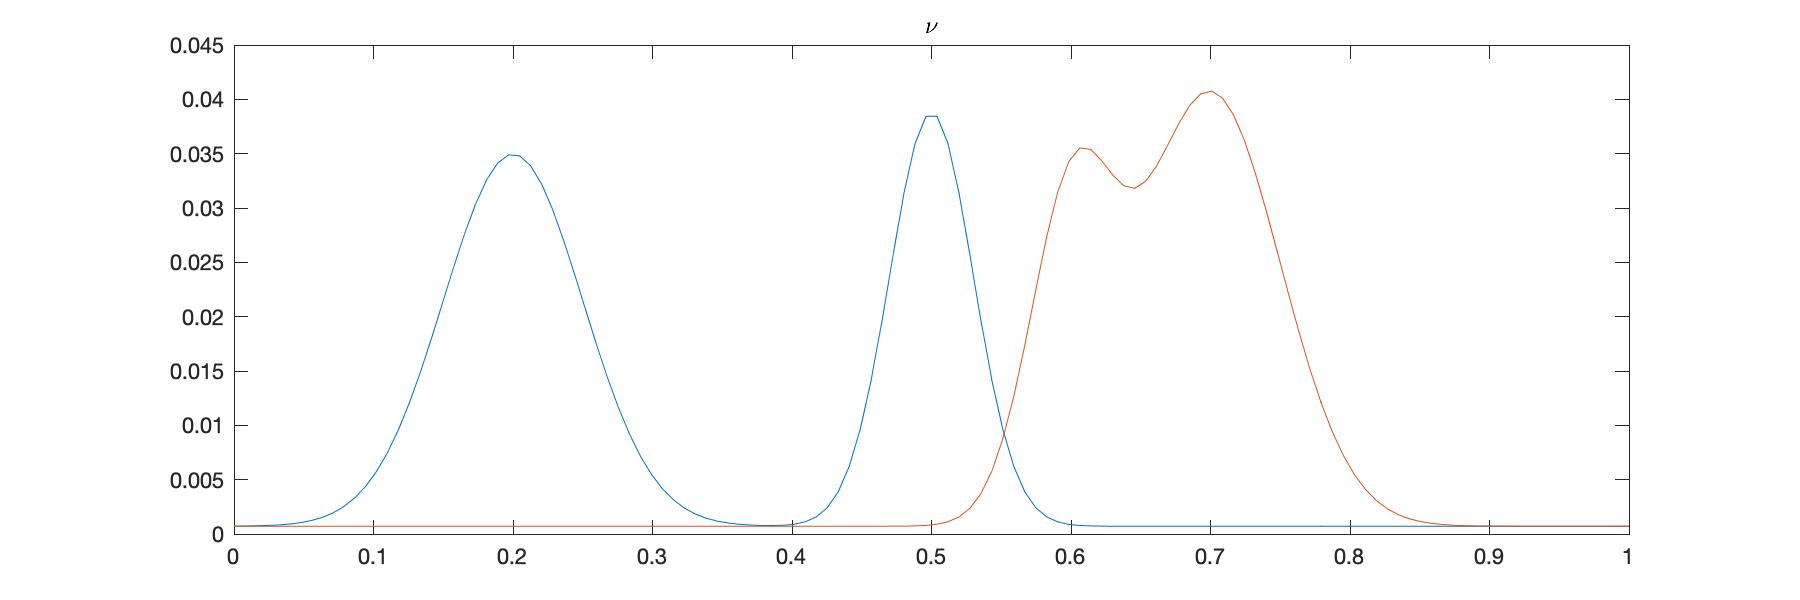
\includegraphics[width=12cm]{final/gmm3.jpg}
\caption{The probability distribution function of two Gaussian mixture models $G_1$ and $G_2$. $G_1$ (blue one) has mean $[0.2,0.5]$, variance $[0.05^2, 0.03^2]$ and component proportion $[0.6, 0.4]$; $G_2$ (red one) has mean $[0.6,0.7]$, variance $[0.03^2, 0.05^2]$ and component proportion $[0.3, 0.7]$. }
\label{gmm3}
\end{figure}

We then take $\epsilon=10^{-2},10^{-3},10^{-4},10^{-5}$. If we use the vanilla Sinkhorn's algorithm \ref{alg:sa} for $\epsilon=10^{-4},10^{-5}$, $K^{\epsilon}$ would be a zero matrix. For Sinkhorn's algorithm with numerical stability \ref{alg:sans}, we take the maximum iteration number to be $10,100,1000,4000$ respectively. For Sinkhorn's algorithm with numerical stability and continuation strategy \ref{alg:sansc}, we take $\alpha=0.1$, $\epsilon_0=\epsilon\times 10^5$ and the maximum iteration number to be $2,20,200,800$ respectively. 

\begin{figure}[!htb]
\centering
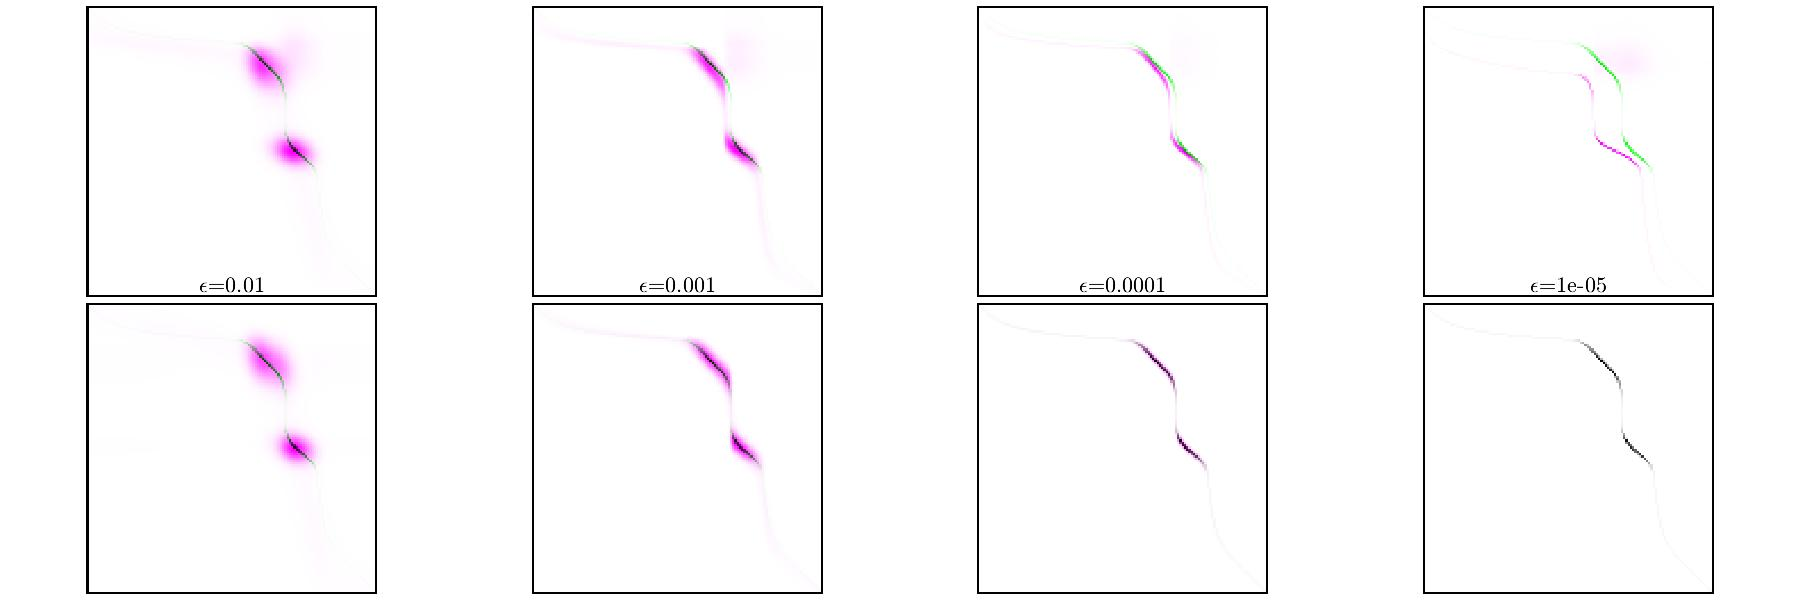
\includegraphics[width=12cm]{final/gmm4.jpg}
	\caption{Impact of $\epsilon$ on the coupling between two gaussian mixture models \ref{gmm1}. From left to right, $\epsilon=10^{-2},10^{-3},10^{-4},10^{-5}$. The upper row is without continuation strategy and the lower row is with continuatation strategy. The purple one is the solution to the entropic regularized LP. The green one is the solution to the original LP.}
\label{gmm4}
\end{figure}

From Figure \ref{gmm4}, we can find that with same iteration number, Sinkhorn's algorithm with numerical stability and continuation strategy converges faster than the one only with numerical stability. This shows that with proper choice of the parameter of continuation, we can achieve acceleration in Sinkhorn's algorithm with continuation strategy.

We then perform a comprehensive numerical experiment on Gaussian mixture model. Detailed parameters and the stopping criterions are listed in Table \ref{param_er}. 

\begin{table}[htbp]
\caption{Perfomance of algorithms for entropic regularization of OT on Gaussian mixture model}
\label{gmm_er}
\centering
\begin{tabular} {|c|c|c|c|c|c|c|c|} 
\hline
\multicolumn{2}{|c|}{ }&\multicolumn{2}{c|}{$\epsilon=10^{-2}$}
&\multicolumn{2}{c|}{$\epsilon=10^{-4}$}
&\multicolumn{2}{c|}{$\epsilon=10^{-6}$}\\
\hline
\multicolumn{2}{|c|}{method}&sinkhorn&ADMM&sinkhorn&ADMM&sinkhorn&ADMM\\\hline
\multirow{4}*{\makecell{$m=128$\\$n=128$}} 
& time(s) & 10.39 & 0.23 & 9.52 & 0.85 & 7.92 & 6.19 \\\cline{2-8}              
& iter & 20000 & 647 & 20000 & 2398 & 20000 & 20000 \\\cline{2-8}               
& objval & 7.25e-02 & 7.24e-02 & 6.77e-04 & 2.19e-03 & 1.76e-04 & 2.32e-04 \\\cline{2-8}                                                                        
& entval & -2.50e-02 & -2.50e-02 & 5.20e-02 & 5.20e-02 & 5.26e-02 & 5.26e-02 \\\cline{2-8}                                                                      
& vltcst & 1.27e-12 & 9.93e-08 & 6.15e-14 & 9.96e-08 & 5.14e-12 & 3.83e-07 \\\hline

\multirow{4}*{\makecell{$m=256$\\$n=256$}} 
& time(s) & 34.53 & 1.34 & 31.96 & 1.90 & 25.48 & 18.53 \\\cline{2-8}           
& iter & 20000 & 1213 & 20000 & 1782 & 20000 & 18203 \\\cline{2-8}              
& objval & 7.27e-02 & 7.26e-02 & 8.55e-04 & 1.85e-03 & 4.94e-04 & 2.74e-04 \\\cline{2-8}                                                                        
& entval & -3.89e-02 & -3.89e-02 & 5.19e-02 & 5.19e-02 & 5.26e-02 & 5.26e-02 \\\cline{2-8}
& vltcst & 1.37e-12 & 9.96e-08 & 1.17e-13 & 9.91e-08 & 3.83e-12 & 9.98e-08 \\\hline

\multirow{4}*{\makecell{$m=512$\\$n=512$}} 
& time(s) & 140.15 & 12.56 & 130.25 & 11.82 & 104.53 & 56.03 \\\cline{2-8}     
& iter & 20000 & 2228 & 20000 & 2100 & 20000 & 9939 \\\cline{2-8}              
& objval & 7.27e-02 & 7.26e-02 & 8.95e-04 & 1.44e-03 & 2.07e-04 & 3.22e-04 \\\cline{2-8}
& entval & -5.28e-02 & -5.28e-02 & 5.17e-02 & 5.17e-02 & 5.26e-02 & 5.26e-02 \\\cline{2-8}
& vltcst & 1.42e-12 & 9.99e-08 & 8.56e-14 & 9.99e-08 & 1.58e-12 & 9.97e-08 \\\hline

\multirow{4}*{\makecell{$m=1024$\\$n=1024$}} 
& time(s) & 692.47 & 99.56 & 658.32 & 86.61 & 557.13 & 144.90 \\\cline{2-8}
& iter & 20000 & 4034 & 20000 & 3523 & 20000 & 5896 \\\cline{2-8}
& objval & 7.27e-02 & 7.24e-02 & 8.79e-04 & 7.20e-04 & 1.84e-04 & 4.07e-04 \\\cline{2-8}
& entval & -6.67e-02 & -6.67e-02 & 5.16e-02 & 5.16e-02 & 5.26e-02 & 5.26e-02 \\\cline{2-8}
& vltcst & 1.29e-12 & 9.99e-08 & 1.30e-13 & 1.00e-07 & 1.49e-12 & 1.00e-07 \\\hline

\end{tabular}
\end{table}
Table \ref{gmm_er} gives the comprehensive numerical results for Gaussian Mixture Model. The setting is same as Figure \ref{gmm1}, except that we test examples for different problem sizes, i.e., we let $N=128, 256, 512, 1024$, respectively. We observe that, in most cases, although `sinkhorn' takes much longer time and more iterations than `ADMM', `sinkhorn' outperforms `ADMM' in both `objval' and `vltcst'. 

\subsubsection{Randomly generated data}
The parameters and the stopping criterions are listed in Table \ref{param_er}. Table \ref{RGD_er} presents numerical results on random generated data. 

\begin{table}[htbp]
\caption{Perfomance of algorithms for entropic regularization of OT on randomly generated data}
\label{RGD_er}
\centering
\begin{tabular} {|c|c|c|c|c|c|c|c|} 
\hline
\multicolumn{2}{|c|}{ }&\multicolumn{2}{c|}{$\epsilon=10^{-2}$}
&\multicolumn{2}{c|}{$\epsilon=10^{-4}$}
&\multicolumn{2}{c|}{$\epsilon=10^{-6}$}\\
\hline
\multicolumn{2}{|c|}{method}&sinkhorn&ADMM&sinkhorn&ADMM&sinkhorn&ADMM\\\hline
\multirow{4}*{\makecell{$m=128$\\$n=128$}} 
& time(s) & 10.06 & 0.82 & 8.36 & 6.16 & 6.84 & 6.21 \\\cline{2-8}             
& iter & 20000 & 2223 & 20000 & 20000 & 20000 & 20000 \\\cline{2-8}            
& objval & 2.40e-04 & 3.18e-04 & 1.23e-03 & -6.35e-06 & 2.54e-03 & -8.73e-06 \\\cline{2-8}                                                                     
& entval & 1.30e+00 & 1.30e+00 & 1.36e+00 & 1.36e+00 & 1.36e+00 & 1.36e+00 \\\cline{2-8}                                                                       
& vltcst & 6.48e-15 & 9.99e-08 & 6.60e-13 & 2.22e-07 & 9.86e-11 & 4.72e-07 \\\hline

\multirow{4}*{\makecell{$m=256$\\$n=256$}} 
& time(s) & 32.66 & 3.23 & 26.86 & 19.88 & 20.49 & 20.46 \\\cline{2-8}         
& iter & 20000 & 3072 & 20000 & 20000 & 20000 & 20000 \\\cline{2-8}            
& objval & 3.16e-04 & 3.49e-04 & 2.36e-03 & -9.92e-06 & 4.52e-03 & -1.24e-05 \\\cline{2-8}                                                                     
& entval & 1.56e+00 & 1.56e+00 & 1.63e+00 & 1.62e+00 & 1.63e+00 & 1.63e+00 \\\cline{2-8}
& vltcst & 2.98e-15 & 9.99e-08 & 7.04e-13 & 5.62e-07 & 1.28e-10 & 6.90e-07 \\\hline

\multirow{4}*{\makecell{$m=512$\\$n=512$}} 
& time(s) & 134.57 & 17.43 & 108.35 & 111.25 & 83.80 & 111.31 \\\cline{2-8}    
& iter & 20000 & 3045 & 20000 & 20000 & 20000 & 20000 \\\cline{2-8}            
& objval & 3.48e-04 & 3.76e-04 & 1.55e-03 & -4.66e-05 & 3.43e-03 & -4.69e-05 \\\cline{2-8}
& entval & 1.49e+00 & 1.49e+00 & 1.57e+00 & 1.57e+00 & 1.57e+00 & 1.57e+00 \\\cline{2-8}
& vltcst & 9.34e-15 & 9.98e-08 & 7.69e-13 & 2.18e-07 & 8.42e-11 & 3.08e-07 \\\hline

\multirow{4}*{\makecell{$m=1024$\\$n=1024$}} 
& time(s) & 692.35 & 99.61 & 568.16 & 497.03 & 472.21 & 495.21 \\\cline{2-8}   
& iter & 20000 & 4040 & 20000 & 20000 & 20000 & 20000 \\\cline{2-8}            
& objval & 2.11e-04 & 2.04e-04 & 1.93e-03 & -1.15e-04 & 3.54e-03 & -1.23e-04 \\\cline{2-8}
& entval & 1.85e+00 & 1.85e+00 & 1.94e+00 & 1.93e+00 & 1.94e+00 & 1.94e+00 \\\cline{2-8}
& vltcst & 1.63e-14 & 9.97e-08 & 1.22e-12 & 2.18e-07 & 1.06e-10 & 2.99e-07 \\\hline

\end{tabular}
\end{table}

We find that the `objval' and `vltcst' of `sinkhorn' is getting worse with the decrease of $\epsilon$. This can be explained by the computation complexity of Sinkhorn's algorithm. As shown in Section 3.2, the $\tau$-approximate solution of the unregularized OT problem takes $O(n^2\log(n)\tau^{-3})$ operations where $\epsilon=\tau/\log(n)$. This means that if we decrease the $\epsilon$ by $0.1$, theoretically we would need $10^3$ times iteration to get a precise solution. Although our improvements of Sinkhorn's algorithm makes it adapt to small $\epsilon$, but the computation is costly. If we want to use Sinkhorn's algorithm to get an approximation solution of the orignial problem \ref{lp}, we should pay attention to choose an appropriate $\epsilon$. 

On the contrary, `ADMM' appears robustness in satisfying constraints within acceptable iteration number. `vltcst' of all test samples are below 1e-06, though it's not comparable to `sinkhorn'. `objval' of ADMM appears to be gradually lower than `prim(M)' when $\epsilon$ decreases. It's worth noting that in `ADMM' we do not apply continuation strategy. In fact, we observe that with the carefully selected $t$, `ADMM' converges quite fast to the optimal value at the beginning, whatever $\epsilon$ is, although vibration is unavoidable in the latter steps. Of course, for $\epsilon$ not large and small or moderate problem sizes, `sinkhorn' performs better than `ADMM'.


\subsubsection{DOTmark}
Detailed parameters are listed in \ref{param_er}. (The stopping rule for `ADMM' changes to $\text{`vltcst'}\leqslant$ 1e-07 or $\text{`iter'}\geqslant$ 2e+04.) Table \ref{DOTmark_er1} and \ref{DOTmark_er2} present numerical results on DOTmark.
\begin{table}[htbp]
\caption{Perfomance of algorithms for entropic regularization of OT on DOTmark Part1}
\label{DOTmark_er1}
\centering
\begin{tabular} {|c|c|c|c|c|c|c|c|} 
\hline
\multicolumn{2}{|c|}{ }&\multicolumn{2}{c|}{$\epsilon=10^{-2}$}
&\multicolumn{2}{c|}{$\epsilon=10^{-4}$}
&\multicolumn{2}{c|}{$\epsilon=10^{-6}$}\\
\hline
Class No.&method &sinkhorn&ADMM&sinkhorn&ADMM&sinkhorn&ADMM\\\hline
\multirow{4}*{1} 
& time(s) & 593.54 & 335.53 & 502.26 & 369.18 & 440.68 & 371.82 \\\cline{
2-8}                                                                            
& iter & 20000 & 13674 & 20000 & 15058 & 20000 & 15062 \\\cline{2-8}        
& objval& 2.01e-02 & 8.30e-04 & 3.36e-02 & 6.52e-04 & 2.11e+00 & 7.27e-04 \\\cline{2-8}                                                             
& entval & 1.78e+01 & 1.74e+01 & 1.81e+01 & 1.75e+01 & 5.44e+01 & 1.75e+01 \\\cline{2-8}                                                             
& vltcst & 2.87e-13 & 2.00e-07 & 2.38e-11 & 2.00e-07 & 6.03e-10 & 2.00e-07 \\\hline 

\multirow{4}*{2} 
& time(s) & 610.36 & 264.70 & 499.11 & 318.66 & 445.02 & 318.45 \\\cline{2-8}                                                                            
& iter & 20000 & 10740 & 20000 & 13021 & 20000 & 13021 \\\cline{2-8}        
& objval & 4.60e-02 & -1.17e-03 & 7.43e-02 & 4.09e-04 & 5.86e+00 & 4.29e-04 \\\cline{2-8}                                                            
& entval & 6.47e+00 & 6.18e+00 & 6.74e+00 & 6.27e+00 & 4.30e+01 & 6.07e+00 \\\cline{2-8}                                                             
& vltcst & 1.46e-13 & 2.00e-07 & 1.69e-11 & 2.00e-07 & 3.80e-10 & 2.00e-07 \\\hline

\multirow{4}*{3} 
& time(s)& 591.98 & 299.63 & 499.19 & 361.14 & 442.04 & 361.33 \\\cline{2-8}
& iter & 20000 & 12206 & 20000 & 14672 & 20000 & 14668 \\\cline{2-8}
& objval & 8.12e-02 & 3.74e-04 & 2.46e-01 & -1.14e-03 & 6.45e+00 & -1.11e-03 \\\cline{2-8}
& entval & 4.32e+00 & 3.99e+00 & 5.07e+00 & 4.07e+00 & 3.03e+01 & 4.07e+00 \\\cline{2-8}
& vltcst & 1.52e-13 & 2.00e-07 & 9.59e-12 & 2.00e-07 & 2.85e-10 & 2.00e-07 \\\hline

\multirow{4}*{4}
& time(s) & 591.00 & 268.63 & 499.50 & 330.66 & 441.70 & 331.92 \\\cline{2-8}
& iter & 20000 & 10923 & 20000 & 13433 & 20000 & 13467 \\\cline{2-8}
& objval & 2.18e-01 & -1.26e-03 & 4.58e-01 & -5.81e-04 & 9.30e+00 & -5.05e-04 \\\cline{2-8}
& entval  & 1.71e+00 & 1.39e+00 & 2.15e+00 & 1.47e+00 & 1.52e+01 & 1.48e+00 \\\cline{2-8}
& vltcst & 1.17e-13 & 2.00e-07 & 6.78e-12 & 2.00e-07 & 2.35e-10 & 2.00e-07 \\\hline

\multirow{4}*{5}
& time(s) & 589.61 & 295.34 & 499.33 & 368.54 & 442.19 & 368.14 \\\cline{2-8}
& iter & 20000 & 12018 & 20000 & 15052 & 20000 & 15047 \\\cline{2-8}
& objval &  8.86e-03 & 8.71e-04 & 3.55e-02 & 9.91e-04 & 2.46e+00 & 9.9
4e-04 \\\cline{2-8}
& entval & 2.15e+01 & 2.13e+01 & 2.22e+01 & 2.14e+01 & 7.41e+01 & 2.14e+01 \\\cline{2-8}
& vltcst & 1.97e-13 & 2.00e-07 & 3.58e-11 & 2.00e-07 & 5.87e-10 & 2.00e-07 \\\hline

\multirow{4}*{6}
& time(s) & 590.35 & 253.97 & 498.56 & 326.70 & 441.70 & 327.49 \\\cline{2-8}
& iter & 20000 & 10339 & 20000 & 13362 & 20000 & 13385 \\\cline{2-8}
& objval & 1.10e-02 & 2.37e-04 & 3.88e-02 & -3.33e-04 & 2.17e+00 & -3.35e-04 \\\cline{2-8}
& entval & 1.93e+01 & 1.91e+01 & 1.99e+01 & 1.92e+01 & 6.09e+01 & 1.92e+01 \\\cline{2-8}
& vltcst & 3.53e-13 & 2.00e-07 & 3.24e-11 & 2.00e-07 & 8.49e-10 & 2.00e-07 \\\hline

\multirow{4}*{7} 
& time(s) & 590.12 & 296.02 & 499.00 & 339.12 & 441.04 & 339.56 \\\cline{2-8}
& iter & 20000 & 12054 & 20000 & 13862 & 20000 & 13877 \\\cline{2-8}
& objval  & 1.60e-02 & 9.12e-04 & 4.17e-02 & -4.18e-04 & 2.82e+00 & -4.48e-04 \\\cline{2-8}
& entval & 1.71e+01 & 1.69e+01 & 1.76e+01 & 1.69e+01 & 6.48e+01 & 1.69e+01 \\\cline{2-8}
& vltcst & 3.62e-13 & 2.00e-07 & 3.62e-11 & 2.00e-07 & 6.20e-10 & 2.00e-07 \\\hline

\end{tabular}
\end{table}
\begin{table}[htbp]
\caption{Perfomance of algorithms for entropic regularization of OT on DOTmark Part2}
\label{DOTmark_er2}
\centering
\begin{tabular} {|c|c|c|c|c|c|c|c|} 
\hline
\multicolumn{2}{|c|}{ }&\multicolumn{2}{c|}{$\epsilon=10^{-2}$}
&\multicolumn{2}{c|}{$\epsilon=10^{-4}$}
&\multicolumn{2}{c|}{$\epsilon=10^{-6}$}\\
\hline
Class No.&method &sinkhorn&ADMM&sinkhorn&ADMM&sinkhorn&ADMM\\\hline

\multirow{4}*{8} 
& time(s) & 604.68 & 273.63 & 502.38 & 374.75 & 441.42 & 374.83 \\\cline{2-8}                                                                            
& iter & 20000 & 11185 & 20000 & 15318 & 20000 & 15323 \\\cline{2-8}        
& objval & 3.30e-02 & 6.25e-04 & 4.21e-02 & -1.95e-04 & 2.01e+00 & -2.27e-04 \\\cline{2-8}                                                           
& entval & 1.12e+01 & 1.08e+01 & 1.13e+01 & 1.09e+01 & 3.27e+01 & 1.09e+01 \\\cline{2-8}                                                             
& vltcst & 5.46e-13 & 2.00e-07 & 1.72e-11 & 2.00e-07 & 8.71e-10 & 2.00e-07 \\\hline

\multirow{4}*{9} 
& time(s) & 603.00 & 249.23 & 501.40 & 299.38 & 439.78 & 264.61 \\\cline{2-8}
& iter & 20000 & 10177 & 20000 & 12241 & 20000 & 10814 \\\cline{2-8}
& objval & 1.69e-05 & 4.17e-05 & 1.69e-05 & -7.33e-05 & 7.96e-01 & 9.68e-05 \\\cline{2-8}
& entval  & 2.43e+01 & 2.43e+01 & 2.44e+01 & 2.44e+01 & 4.38e+01 & 2.24e+01 \\\cline{2-8}
& vltcst   & 6.59e-13 & 1.98e-07 & 2.73e-11 & 1.99e-07 & 5.95e-10 & 1.99e-07 \\\hline

\multirow{4}*{10}
& time(s) & 590.49 & 237.95 & 500.10 & 281.92 & 441.94 & 282.65 \\\cline{2-8}
& iter & 20000 & 9693 & 20000 & 11524 & 20000 & 11549 \\\cline{2-8}
& objval & 4.20e-01 & 1.98e-03 & 1.25e+00 & -1.02e-03 & 7.78e+00 & -1.21e-04 \\\cline{2-8}
& entval & 9.22e-01 & 6.25e-01 & 1.60e+00 & 7.08e-01 & 6.23e+00 & 7.09e-01 \\\cline{2-8}
& vltcst & 2.17e-13 & 2.00e-07 & 2.16e-12 & 2.00e-07 & 1.18e-10 & 2.00e-07 \\\hline

\end{tabular}
\end{table}

Same as before, `objval' and `vltcst' of `sinkhorn' is getting worse with the decrease of $\epsilon$. All of the results are within 1e-09 in `vltcst', but `objval' deteriorate rapidly when $\epsilon$ decreases. This can be again explained by the computation complexity of Sinkhorn's algorithm. 

'ADMM' can achieve relatively lower objective value on average, and need moderate iterations before `vltcst' arrives at a threshold. The performance is similar to random generated data setting with larger problem sizes. We should note that due to the different problem structures, it seems difficult sometimes for `ADMM' to outperform `prim(M)'.

\subsubsection{Ellipse Example \& Caffarelli's Example}
\begin{table}[htbp]
\caption{Perfomance of algorithms for entropic regularization of OT on Ellipse Example}
\label{ellipse_er}
\centering
\begin{tabular} {|c|c|c|c|c|c|c|c|} 
\hline
\multicolumn{2}{|c|}{ }&\multicolumn{2}{c|}{$\epsilon=10^{-2}$}
&\multicolumn{2}{c|}{$\epsilon=10^{-4}$}
&\multicolumn{2}{c|}{$\epsilon=10^{-6}$}\\
\hline
\multicolumn{2}{|c|}{method}&sinkhorn&ADMM&sinkhorn&ADMM&sinkhorn&ADMM\\\hline
\multirow{4}*{\makecell{$m=128$\\$n=128$}} 
& time(s) & 10.04 & 0.36 & 8.91 & 6.23 & 7.18 & 6.21 \\\cline{2-8}              
& iter & 20000 & 984 & 20000 & 20000 & 20000 & 20000 \\\cline{2-8}              
& objval & 1.77e-03 & 2.24e-03 & 5.91e-04 & 1.58e-05 & 4.66e-03 & 7.81e-06 \\\cline{2-8}                                                                        
& entval & 2.50e+00 & 2.50e+00 & 2.57e+00 & 2.57e+00 & 2.58e+00 & 2.57e+00 \\\cline{2-8}                                                                        
& vltcst & 1.90e-14 & 9.95e-08 & 3.11e-13 & 3.85e-07 & 9.03e-11 & 5.63e-07 \\\hline  

\multirow{4}*{\makecell{$m=256$\\$n=256$}} 
& time(s) & 33.01 & 0.81 & 29.70 & 19.50 & 22.52 & 20.14 \\\cline{2-8}          
& iter & 20000 & 705 & 20000 & 19370 & 20000 & 20000 \\\cline{2-8}              
& objval & 2.37e-03 & 2.72e-03 & 3.32e-04 & 2.71e-05 & 1.58e-03 & 1.97e-05 \\\cline{2-8}                                                                        
& entval & 2.40e+00 & 2.40e+00 & 2.48e+00 & 2.48e+00 & 2.49e+00 & 2.48e+00 \\\cline{2-8}
& vltcst & 1.42e-14 & 9.91e-08 & 9.55e-13 & 9.97e-08 & 9.77e-11 & 2.43e-07 \\\hline

\multirow{4}*{\makecell{$m=512$\\$n=512$}} 
& time(s) & 134.58 & 3.57 & 119.84 & 91.35 & 91.55 & 112.25 \\\cline{2-8}
& iter & 20000 & 637 & 20000 & 16276 & 20000 & 20000 \\\cline{2-8}
& objval & 3.06e-03 & 3.27e-03 & 2.80e-04 & 3.83e-05 & 1.51e-03 & 1.62e-05 \\\cline{2-8}
& entval & 2.19e+00 & 2.19e+00 & 2.28e+00 & 2.28e+00 & 2.28e+00 & 2.28e+00 \\\cline{2-8}
& vltcst & 1.37e-14 & 9.92e-08 & 1.19e-12 & 9.99e-08 & 1.42e-10 & 2.36e-07 \\\hline

\multirow{4}*{\makecell{$m=1024$\\$n=1024$}} 
& time(s) & 677.72 & 15.72 & 625.73 & 386.85 & 514.66 & 491.65 \\\cline{2-8}
& iter & 20000 & 641 & 20000 & 15739 & 20000 & 20000 \\\cline{2-8}
& objval & 3.40e-03 & 3.48e-03 & 7.94e-05 & -1.92e-05 & 1.61e-03 & -3.87e-05 \\\cline{2-8}
& entval & 2.15e+00 & 2.15e+00 & 2.25e+00 & 2.25e+00 & 2.26e+00 & 2.25e+00 \\\cline{2-8}
& vltcst & 1.37e-14 & 1.00e-07 & 7.50e-13 & 9.99e-08 & 1.30e-10 & 1.46e-07 \\\hline

\end{tabular}
\end{table}
\begin{table}[htbp]
\caption{Perfomance of algorithms for entropic regularization of OT on Caffarelli's Example}
\label{caff_er}
\centering
\begin{tabular} {|c|c|c|c|c|c|c|c|} 
\hline
\multicolumn{2}{|c|}{ }&\multicolumn{2}{c|}{$\epsilon=10^{-2}$}
&\multicolumn{2}{c|}{$\epsilon=10^{-4}$}
&\multicolumn{2}{c|}{$\epsilon=10^{-6}$}\\
\hline
\multicolumn{2}{|c|}{method}&sinkhorn&ADMM&sinkhorn&ADMM&sinkhorn&ADMM\\\hline
\multirow{4}*{\makecell{$m=128$\\$n=128$}} 
& time(s) & 7.61 & 0.50 & 6.76 & 4.64 & 5.58 & 4.66 \\\cline{2-8}               
& iter & 20000 & 1777 & 20000 & 20000 & 20000 & 20000 \\\cline{2-8}             
& objval & 1.03e-03 & 1.45e-03 & 5.04e-04 & 9.71e-06 & 4.01e-04 & 6.89e-06 \\\cline{2-8}                                                                        
& entval & 3.93e+00 & 3.93e+00 & 4.00e+00 & 4.00e+00 & 4.00e+00 & 4.00e+00 \\\cline{2-8}                                                                        
& vltcst & 9.94e-15 & 9.98e-08 & 2.81e-12 & 1.63e-07 & 2.12e-10 & 2.94e-07 \\\hline

\multirow{4}*{\makecell{$m=256$\\$n=256$}} 
& time(s) & 21.63 & 0.84 & 19.52 & 13.12 & 15.29 & 13.09 \\\cline{2-8}          
& iter & 20000 & 1154 & 20000 & 20000 & 20000 & 20000 \\\cline{2-8}             
& objval & 1.40e-03 & 1.90e-03 & 4.87e-04 & 1.32e-05 & 8.98e-04 & 1.18e-05 \\\cline{2-8}                                                                        
& entval & 3.93e+00 & 3.93e+00 & 4.00e+00 & 4.00e+00 & 4.01e+00 & 4.00e+00 \\\cline{2-8}
& vltcst & 1.18e-14 & 9.95e-08 & 1.47e-12 & 1.67e-07 & 1.88e-10 & 2.37e-07 \\\hline

\multirow{4}*{\makecell{$m=512$\\$n=512$}} 
& time(s) & 83.29 & 2.20 & 74.29 & 68.36 & 55.97 & 68.35 \\\cline{2-8}
& iter & 20000 & 644 & 20000 & 20000 & 20000 & 20000 \\\cline{2-8}
& objval & 1.73e-03 & 2.25e-03 & 1.40e-03 & 1.18e-05 & 1.78e-03 & 9.34e-06 \\\cline{2-8}
& entval & 3.92e+00 & 3.92e+00 & 4.01e+00 & 4.00e+00 & 4.01e+00 & 4.01e+00 \\\cline{2-8}
& vltcst & 1.44e-14 & 9.97e-08 & 1.21e-12 & 1.28e-07 & 1.70e-10 & 1.98e-07 \\\hline

\multirow{4}*{\makecell{$m=1024$\\$n=1024$}} 
& time(s) & 428.49 & 11.31 & 390.39 & 256.87 & 320.54 & 321.15 \\\cline{2-8}
& iter & 20000 & 704 & 20000 & 16004 & 20000 & 20000 \\\cline{2-8}
& objval & 2.01e-03 & 2.19e-03 & 6.65e-04 & 7.60e-06 & 1.32e-03 & -1.46e-05 \\\cline{2-8}
& entval & 3.90e+00 & 3.90e+00 & 4.00e+00 & 4.00e+00 & 4.00e+00 & 4.00e+00 \\\cline{2-8}
& vltcst & 1.67e-14 & 9.86e-08 & 1.83e-12 & 9.99e-08 & 2.17e-10 & 1.48e-07 \\\hline

\end{tabular}
\end{table}
Table \ref{param_er} lists the detailed parameters.Table \ref{ellipse_er} and Table \ref{caff_er} present numerical results for Ellipse Example and Caffarelli's Example, respectively. Through our previous experiments, we observe that with the decrease of $\epsilon$, `ADMM' does not require so much increase of computational complexity as `sinkhorn'. This can be explained by the limit when $\epsilon\to0$. When $\epsilon\to0$, `ADMM' reduce to ADMM for the primal problem \ref{lp}. But with $\epsilon\to0$, we have shown in Section 3.3.1 that `sinkhorn' will diverge due to the loss of strong convexity. And with the decrease of $\epsilon$, the strong convexity of problem \ref{equ:kl} decreases. This also explains why `sinkhorn' requires such enormous iterations to find the optimal solution. In summary, we shall use `sinkhorn' to solve the entropic regularization of OT \ref{equ:kl} with moderate $\epsilon$. With large $\epsilon$, we shall use the original Sinkhorn's algorithm \ref{alg:sa} because it is faster in computation. `ADMM' seems to be suitable to arbitrary small $\epsilon$. 
